\documentclass[pdftex,aspectratio=169]{beamer}

% Setup UTF-8 encoding
\usepackage[utf8]{inputenc}
\usepackage[T1]{fontenc}

%\usepackage{flashmovie}

% Setup beamer look theme
\mode<presentation>
{
	\useinnertheme{rectangles}
	\useoutertheme{infolines}
%	\usecolortheme{crane}
%	\usecolortheme{dove}
	\usecolortheme{seagull}
	\setbeamertemplate{navigation symbols}{}
}

% Use nicer font
\usepackage{palatino}
\usepackage{palatino,graphics,array}


% Setup czech language
\usepackage[czech]{babel}

% Include usefull packages
\usepackage{graphics}

% Include hyperlinks support
\usepackage{hyperref}
\hypersetup{colorlinks=true,linkcolor=black,urlcolor=black,unicode=true}

% Add support for simple URLs
\usepackage{url}

\usepackage{tikz}

\usepackage{verbatim}
\usetikzlibrary{arrows,shapes}
\usetikzlibrary{mindmap,trees}


% Commands for CC license
\newcommand{\CcLongnameByNcSa}{\href{http://creativecommons.org/licenses/by-nc-sa/3.0/cz/}{Attribution-Noncommercial-ShareAlike}}
\newcommand{\CcImageBy}[1]{
\includegraphics[scale=#1]{graphics/cc-by-white.pdf}}
\newcommand{\CcImageNc}[1]{
\includegraphics[scale=#1]{graphics/cc-nc-white.pdf}}
\newcommand{\CcImageSa}[1]{
\includegraphics[scale=#1]{graphics/cc-sa-white.pdf}}
\newcommand{\CcGroupByNcSa}[2]{\CcImageBy{#1}\hspace*{#2}\CcImageNc{#1}\hspace*{#2}\CcImageSa{#1}}




\title{Quest for the Holy Grail}
\subtitle{quantifying the quality of parallel job schedules}
\author[]{Mgr.~Šimon~Tóth}
\institute[FI@MU]{Faculty of Informatics @ Masaryk University}
\date{\today}

\newcommand{\CcNote}[1]{% longname
	Licensed under: \textit{Creative Commons #1 3.0 License}.%
}

% odkazy na konkretni publikace
% user-driven skupiny
% fairness skupiny

\begin{document}
\begin{frame}
	\titlepage
	\vfill
	\begin{center}
		\CcGroupByNcSa{0.33}{0.95ex}\\ {\tiny\CcNote{\CcLongnameByNcSa}}
		\vspace*{2ex}
	\end{center}
\end{frame}

% This will be a talk about measuring quality.
% But to put you all into perspective I will start with introducing the parallel job scheduling problem,
% and even before that lets just start by introducing the Czech National Grid.

% Some of you may not know this, but we do have a national grid here in Czech Republic.
% It's free to use for non-commercial resear purposes, so you can all sing up and use it.
% And you probably should be interested, not just because we have some interesting hardware that you can use:
% like GPU clusters, clusters with infiniband for high performance parallel computations, or machines with upto 1TB of memory.
% But we also have a lot of very expensive software that you can all use for your research.
% metavo.metacentrum.cz

\section{Introduction}
\subsection{Czech National Grid}

\begin{frame}
	\frametitle{Czech National Grid}
	\begin{itemize}
		\item available for non-commercial research \pause
		\item interesting hardware \pause
		\begin{itemize}
			\item GPU clusters
			\item clusters with infiniband
			\item machines with up to 1TB RAM
		\end{itemize} \pause
		\item a lot of very expensive and useful software
	\end{itemize}
	\url{http://metavo.metacentrum.cz}
\end{frame}

% That was the advertising part of my presentation, so lets move to the real content.
% Let's talk about the parallel job scheduling problem, which is the official term for planning computational jobs onto machines.


\subsection{Parallel job scheduling problem}

\begin{frame}
	\frametitle{Parallel job scheduling problem}
	\begin{tikzpicture}[auto,
		singlejob/.style = {rectangle, minimum height = 1cm, minimum width = 2cm, fill=blue!20, thick, outer sep=0pt, inner sep=0pt, text centered},
		doublejob/.style = {rectangle, minimum height = 1cm, minimum width = 4.1cm, fill=blue!20, thick, inner sep = 0pt, text centered}
	]
		\matrix[column sep=0.1cm, row sep=0.1cm, ampersand replacement=\& ] {
			\node[rectangle, minimum height = 1cm, minimum width = 1cm ] (user1) { $User_1$ }; \\
			\node[rectangle, minimum height = 1cm, minimum width = 1cm ] (user2) { $User_2$ }; \\
		};
		\node[draw, singlejob, minimum width = 4.5cm, right=0.1cm of user1] (job1) {$Job_1$};
		\node[draw, singlejob, minimum width = 1.8cm, right=0.1cm of job1] {$Job_2$};
		\node[draw, singlejob, minimum width = 2.3cm, right=0.1cm of user2] (job3) {$Job_3$};
		\node[draw, singlejob, minimum width = 1.6cm, right=0.1cm of job3] (job4) {$Job_4$};
		\node[draw, singlejob, minimum width = 1.2cm, right=0.1cm of job4] {$Job_5$};
	\end{tikzpicture}
\end{frame}

\begin{frame}
	\frametitle{Parallel job scheduling problem}
	\begin{tikzpicture}[auto,
		singlejob/.style = {rectangle, minimum height = 1cm, minimum width = 2cm, fill=blue!20, thick, outer sep=0pt, inner sep=0pt, text centered},
		doublejob/.style = {rectangle, minimum height = 1cm, minimum width = 4.1cm, fill=blue!20, thick, inner sep = 0pt, text centered}
	]
		\matrix[column sep=0.1cm, row sep=0.1cm, ampersand replacement=\& ] {
			\node[rectangle, minimum height = 1cm, minimum width = 1cm ] (mach1) { $Resc_1$ }; \\
			\node[rectangle, minimum height = 1cm, minimum width = 1cm ] (mach2) { $Resc_2$ }; \\
			\node[rectangle, minimum height = 1cm, minimum width = 1cm ] (mach3) { $Resc_3$ }; \\
		};
		\node[draw, singlejob, minimum width = 4.5cm, right=0.1cm of mach2] (job1) {$Job_1$};
		\node[draw, singlejob, minimum width = 2.3cm, right=0.1cm of mach1] (job3) {$Job_3$};
		\node[draw, singlejob, minimum width = 1.6cm, right=0.1cm of mach3] (job4) {$Job_4$};
		\node[draw, singlejob, minimum width = 1.2cm, right=0.1cm of job3] (job5) {$Job_5$};
		\node[draw, singlejob, minimum width = 1.8cm, right=0.1cm of job4] (job2){$Job_2$};
	\end{tikzpicture}
\end{frame}

\subsection{Specifics of GRID}

\begin{frame}
	\frametitle{Problem specifics in GRID context}
	\begin{itemize}
		\item multi-dimensional
		\begin{itemize}
			\item each job can request a large set of resources
			\item CPU, Memory, GPU, Scratch, Licenses,...
		\end{itemize}
		\item on-line
		\begin{itemize}
			\item jobs are not known until they arrive into the system
			\item at any time any amount of jobs from any user can arrive
		\end{itemize}
		\item non-clairvoyant
		\begin{itemize}
			\item we only have upper bounds for job run times
			\item jobs appearing as 24 hour long can easily end in 10 minutes
		\end{itemize}
	\end{itemize}
\end{frame}


% In the context of grid scheduling, we are working with an online variant of the problem.
% This simply means that new jobs arrive at any time and the system has now knowledge of jobs that haven't yet arrived into the system.
% This has huge implications on scheduling.
% For one, providing high priority access to machines is big issue, since the high priority jobs can arrive at any time, we would have to keep these machines empty.

% The problem is also non-clairvoirant, which means that while we know upper bound for the length of the job (after this length the job will be terminated)
% we don't know the actuall length. This leads to many issues when constructing a schedule, since a job with upper bound 24 hours can easily end in under 10 minutes.

\section{Quality}
\subsection{Standard metrics vs. quality}
% how did that happen?
% what does that mean?

\begin{frame}
	\frametitle{Wait-time and Slowdown}
	\begin{itemize}
		\item most commonly used "quality" indicators
		\item both suffer from similar flaws
		\begin{itemize}
			\item large sets of jobs from single user
			\item different representations of equivalent requests
		\end{itemize}
	\end{itemize}
\end{frame}

\begin{frame}
	\frametitle{Example of bad evaluation}
	\begin{tikzpicture}[auto,
		singlejob/.style = {rectangle, minimum height = 1cm, minimum width = 2cm, fill=blue!20, thick, outer sep=0pt, inner sep=0pt, text centered},
		doublejob/.style = {rectangle, minimum height = 1cm, minimum width = 4.1cm, fill=blue!20, thick, inner sep = 0pt, text centered}
	]
		\matrix[column sep=0.1cm, row sep=0.1cm, ampersand replacement=\& ] {
			\node[rectangle, minimum height = 1cm, minimum width = 1cm ] { $Resc_1$ };\&
			\node[draw, singlejob] {$Job_1$};\& \node[draw, singlejob] {$Job_2$};\&
			\node[singlejob] (j51) {}; \& \node[singlejob] (j52) {}; \\

			\node[rectangle, minimum height = 1cm, minimum width = 1cm ] { $Resc_2$ };\&
			\node[draw, singlejob] {$Job_3$};\& \node[draw, singlejob] {$Job_4$}; \&
			\node[singlejob] (j61) {}; \& \node[singlejob] (j62) {}; \\
		};
		\node[draw,doublejob,onslide={<2->{fill=red!20}}] (outer) [fit=(j51) (j52),label=center:$Job_5$] {};
		\node[draw,doublejob,onslide={<2->{fill=red!20}}] (outer) [fit=(j61) (j62),label=center:$Job_6$] {};
	\end{tikzpicture}
\end{frame}


\subsection{Concept of fairness}

\begin{frame}
	\frametitle{Fairness}
	\begin{itemize}
		\item many different representations
		\item commonly used approach is fairshare
		\begin{itemize}
			\item priority balancing algorithm
			\item using the system decreases priority
		\end{itemize}
	\end{itemize}

	\begin{align*}
	& \forall i; \lim_{time \to \infty} Usage(User_i) = TotalUsage \times DesignatedFraction(User_i)
	\end{align*}
\end{frame}

\section{Quantifying the quality}
\subsection{The model}

% So to construct the model we really need to come back to the fundamentals.
% When do we consider a generated schedule good enough.
% Well, the most fundamental aspect is the satisfaction of users.
% When the users are satisfied, the schedule is good enough.

\begin{frame}
	\frametitle{Fundamentals}
	\begin{itemize}
		\item quality based of user satisfaction
		\item modeling user expectations
	\end{itemize}
\end{frame}

\begin{frame}
	\frametitle{The model}
	\begin{itemize}
		\item each user given "bandwidth"
		\begin{itemize}
			\item CPU $8\frac{core}{second}$
			\item memory $16\frac{GB}{second}$
		\end{itemize}
		\item for each job a deadline is calculated according to available bandwidth
	\end{itemize}
\end{frame}

\begin{frame}
	\frametitle{Deadlines example}
	4 jobs
	\begin{itemize}
		\item 4 CPU cores
		\item 8 GB RAM
		\item 4 hour runtime
	\end{itemize}
	Deadlines:
	\begin{itemize}
		\item 4 hours for first and second job
		\item 8 hours for third and fourth job
	\end{itemize}
\end{frame}

\section{Examples of results}
\subsection{Comparing different simple algorithms}

\begin{frame}
	\frametitle{Alea - the Grid Simulation Environment}
	\begin{itemize}
		\item created by RNDr. Dalibor Klusáček, Ph.D.
		\item uses real data sets from CERIT and MetaCentrum
	\end{itemize}
\end{frame}

\begin{frame}
	\frametitle{Scheduling algorithms}
	\begin{itemize}
		\item trivial FIFO
		\item FIFO with backfilling
		\item combinations with fairshare variants
	\end{itemize}
\end{frame}

\begin{frame}
	\frametitle{Overview graphs}
	\begin{center}
	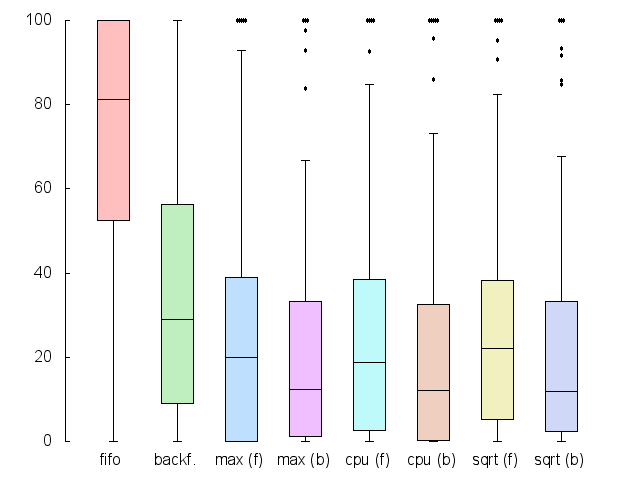
\includegraphics[width=0.6\textwidth]{perc_deadline.png}
	\end{center}
\end{frame}

\begin{frame}
	\frametitle{Trivial FIFO}
	\begin{center}
	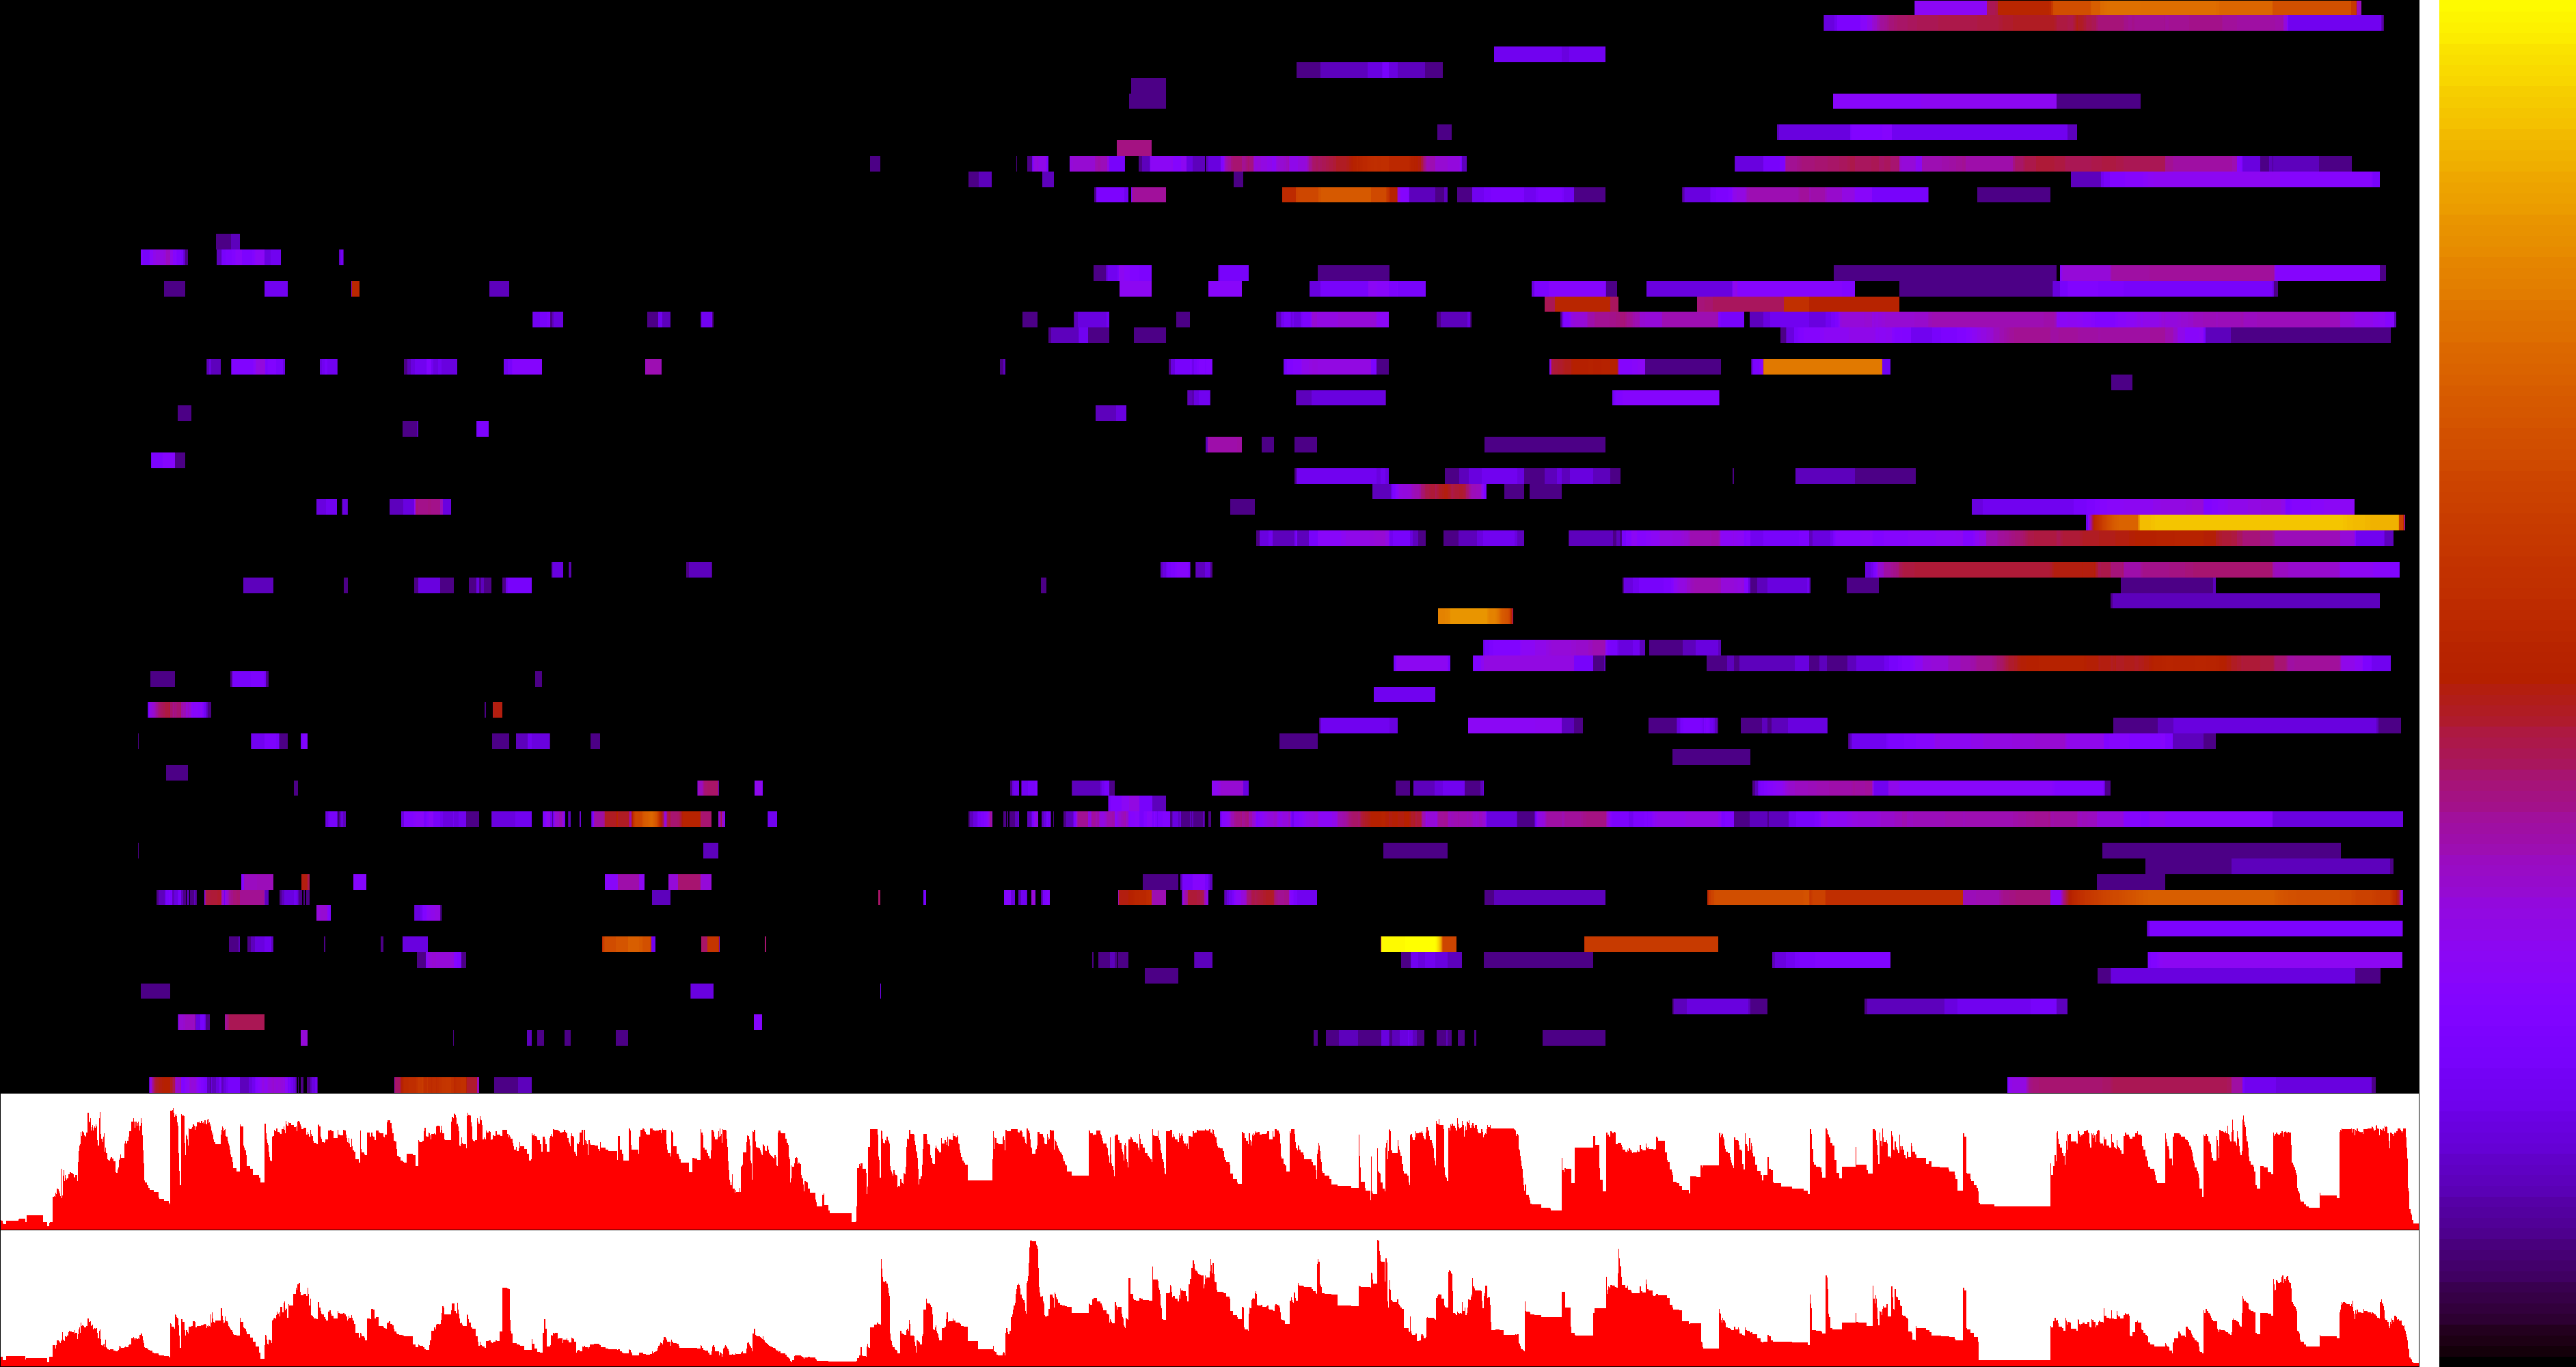
\includegraphics[width=0.85\textwidth]{none_fifo.png}
	\end{center}
\end{frame}

\begin{frame}
	\frametitle{FIFO with backfilling}
	\begin{center}
	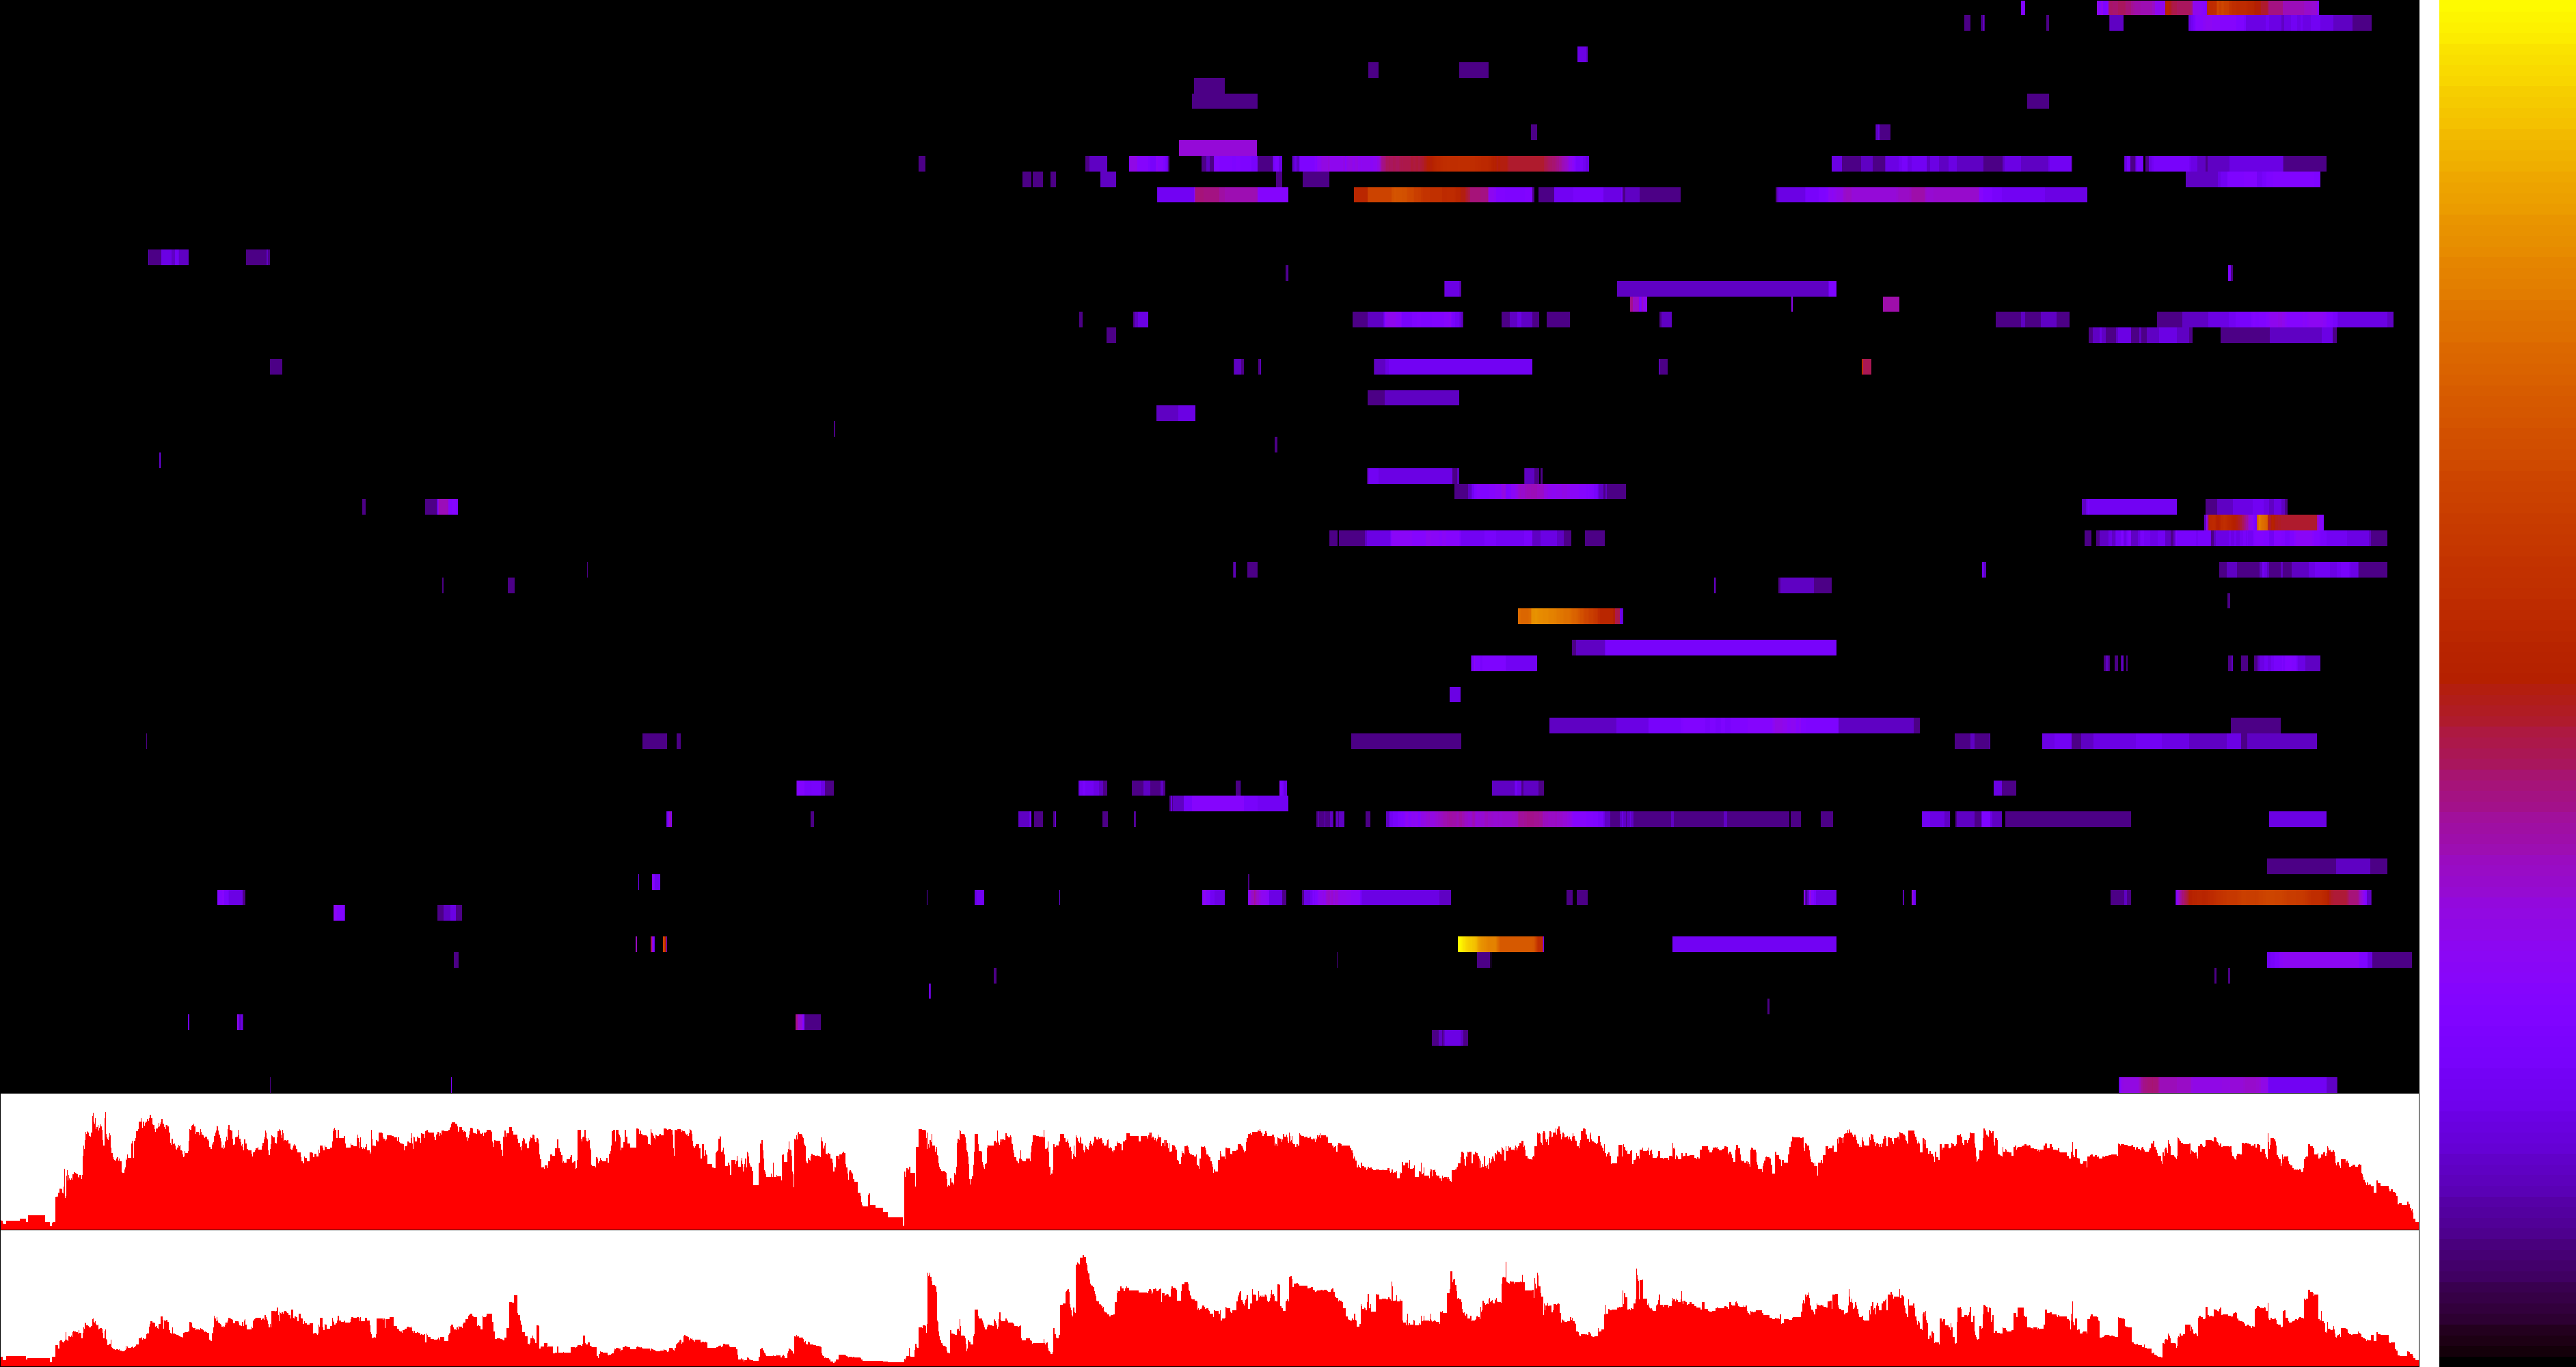
\includegraphics[width=0.85\textwidth]{none_backfill.png}
	\end{center}
\end{frame}

\begin{frame}
	\frametitle{FIFO with fairshare}
	\begin{center}
	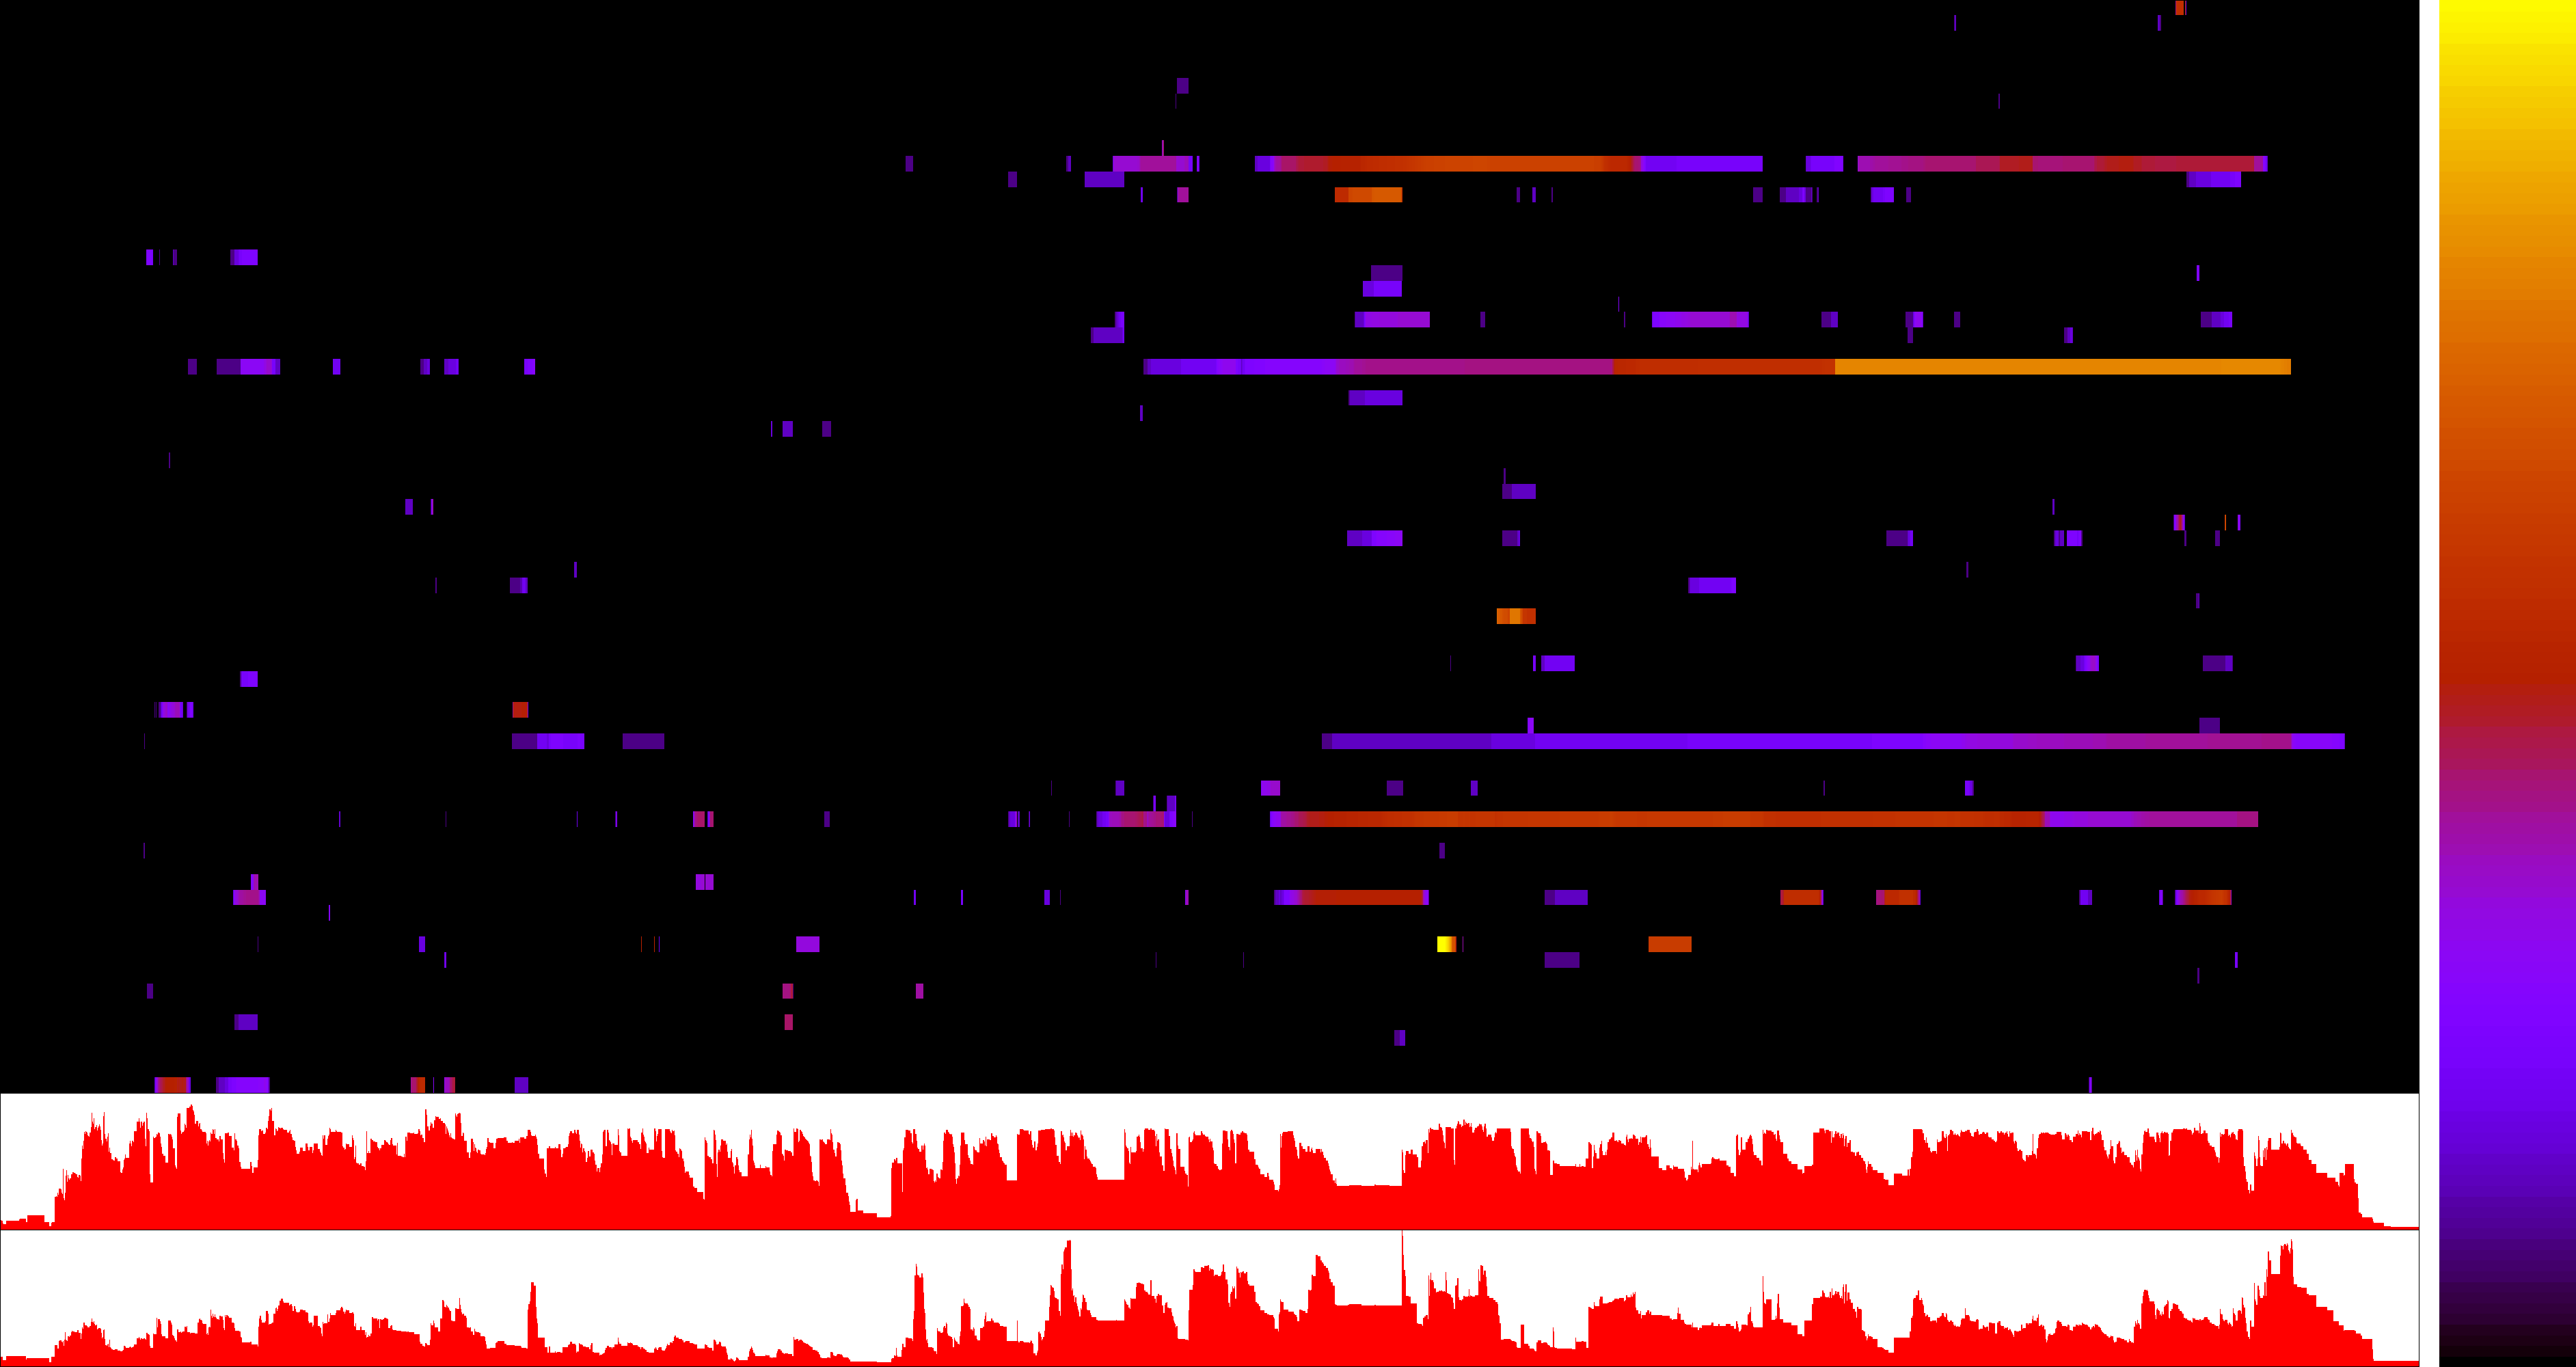
\includegraphics[width=0.85\textwidth]{max_fifo.png}
	\end{center}
\end{frame}

\begin{frame}
	\frametitle{Fairshare and backfilling}
	\begin{center}
	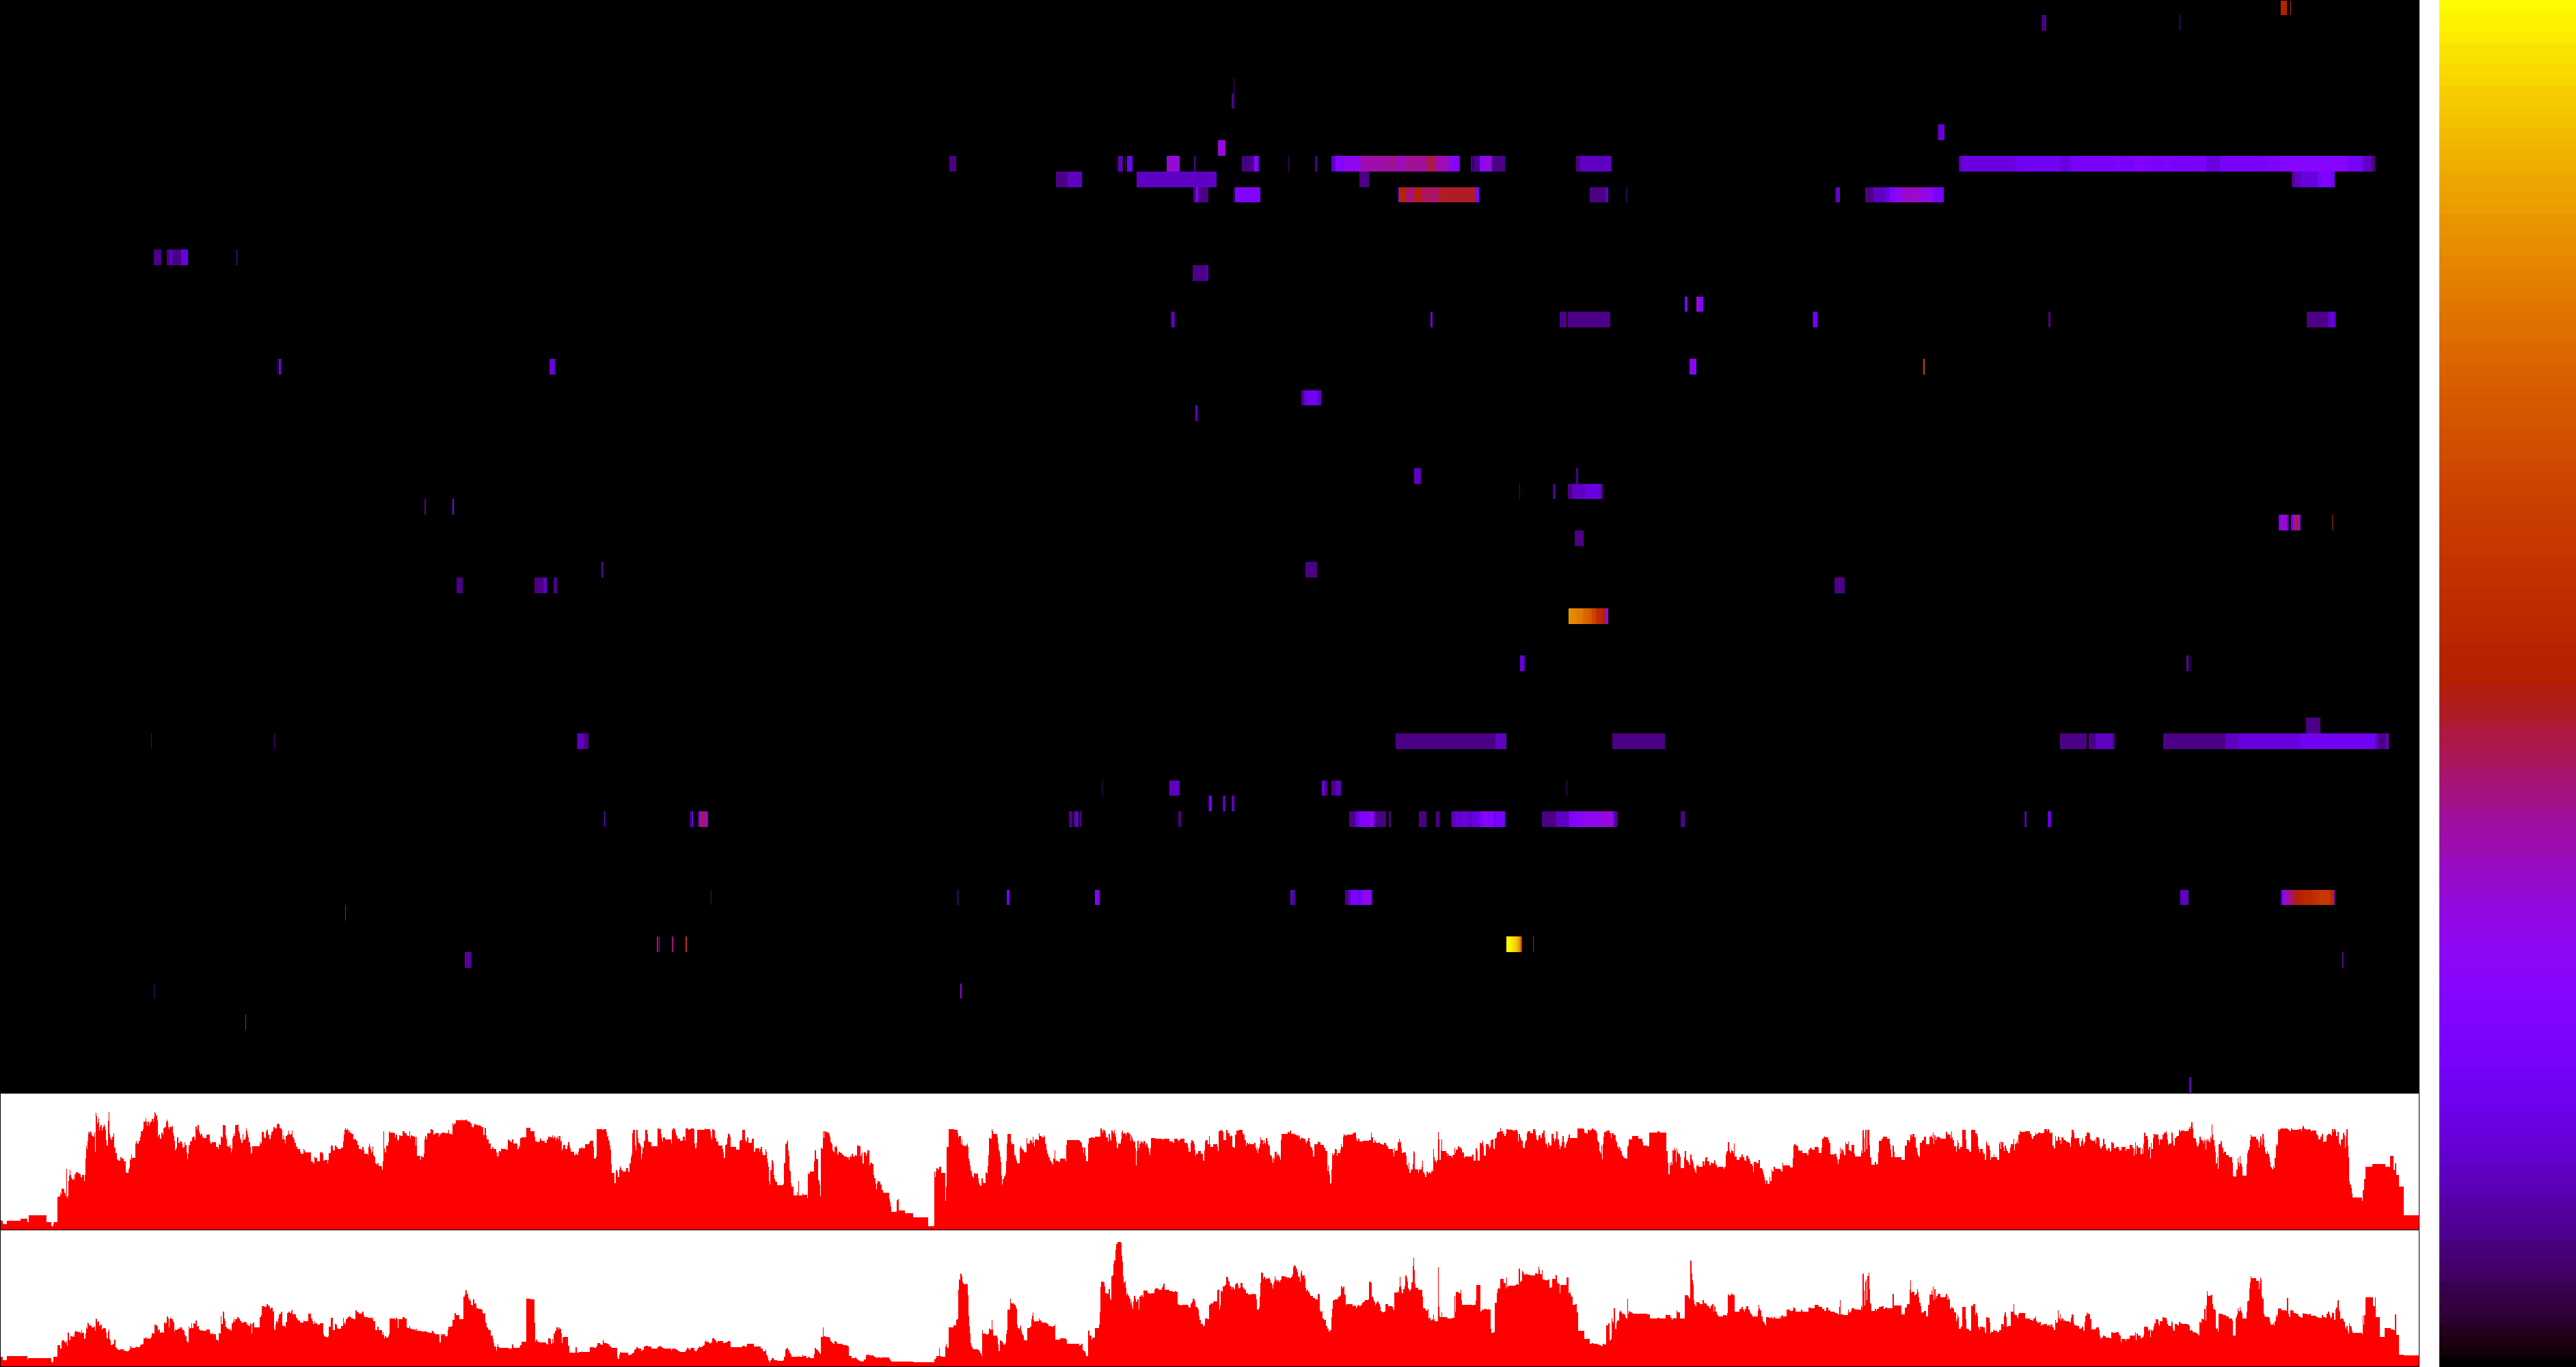
\includegraphics[width=0.85\textwidth]{max_backfill.png}
	\end{center}
\end{frame}

\begin{frame}
	\frametitle{Trivial FIFO}
	\begin{center}
	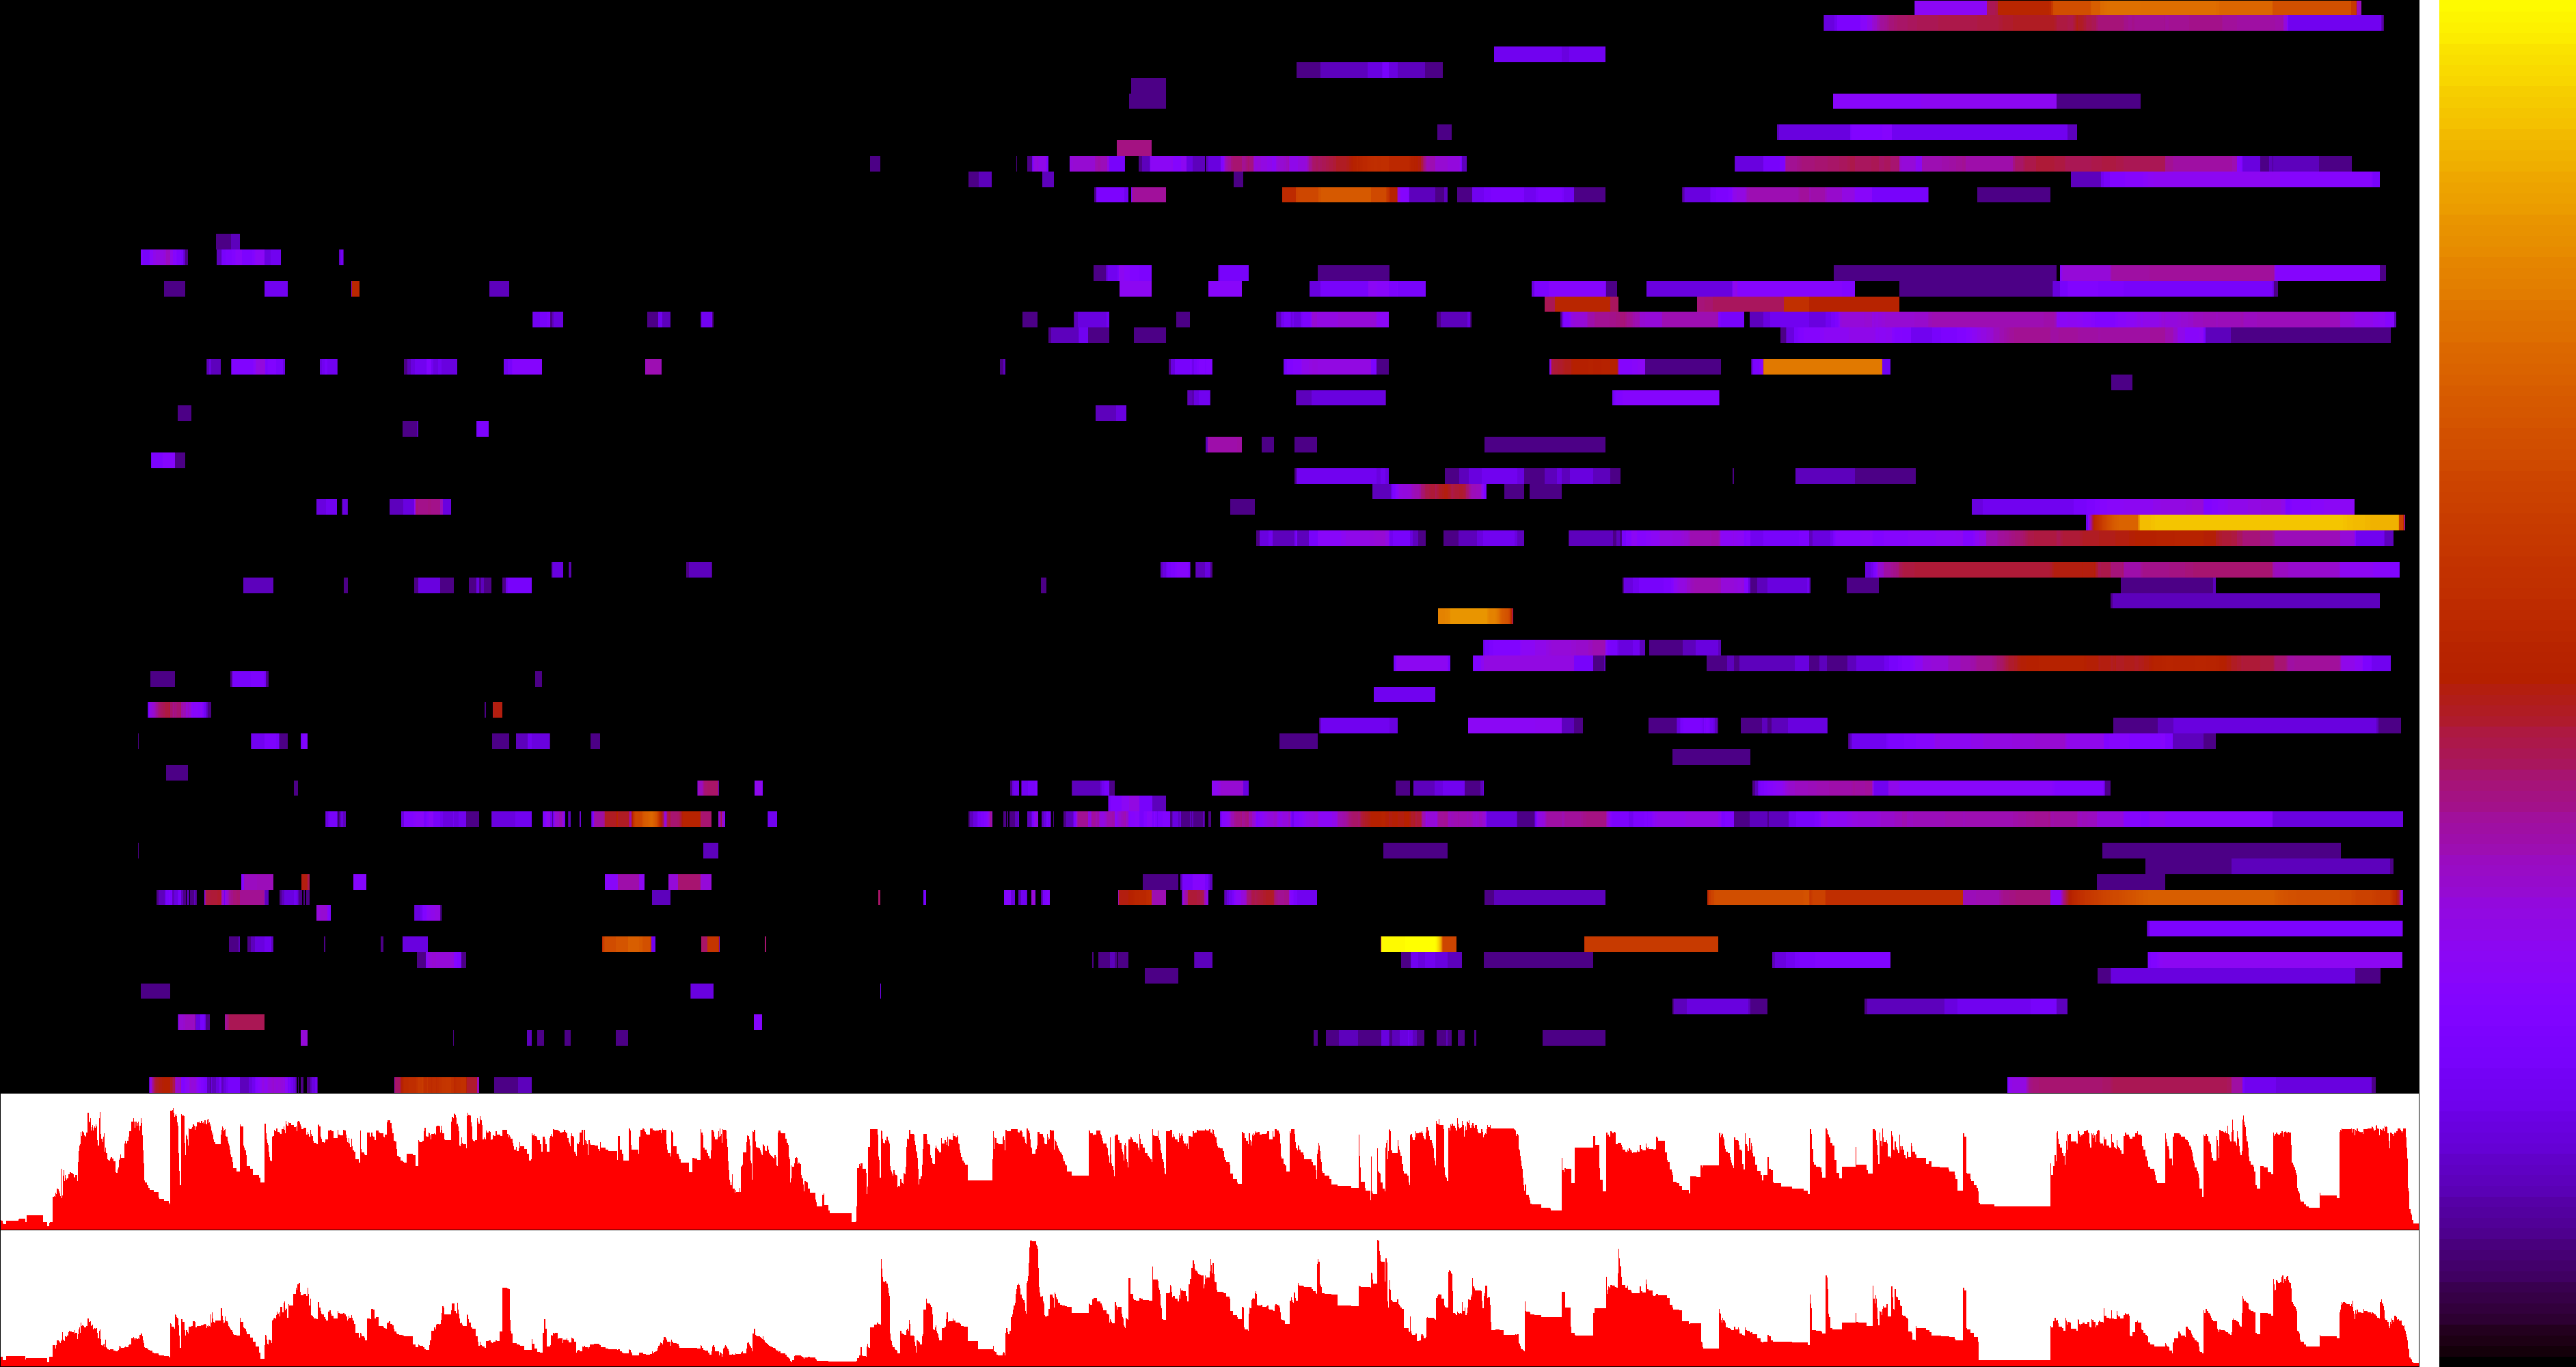
\includegraphics[width=0.85\textwidth]{none_fifo.png}
	\end{center}
\end{frame}

\subsection{Future work}

\begin{frame}
	\frametitle{Future work}
	\begin{itemize}
		\item users with different priorities \pause
		\item users with different tolerance towards deadline violation \pause
		\item users with special access to particular machines
	\end{itemize}
\end{frame}

\section{Conclusion}
\subsection{Summary}

\begin{frame}
	\frametitle{Summary}
	\begin{itemize}
		\item parallel job scheduling in grids \pause
		\item measuring quality of algorithms for job scheduling \pause
		\item model for quantifying the quality schedules \pause
		\item examples of real measurements
	\end{itemize}
\end{frame}

\subsection{The End}

\begin{frame}
	\hspace{0.7cm}
		
\includegraphics[width=0.2\textwidth]{filogo.pdf}
	\hspace{1cm}
	\begin{minipage}[b]{0.3\textwidth}
		
\includegraphics[width=\textwidth]{cesnet-logo-800.png}\newline
		
\includegraphics[width=\textwidth]{metalogo1.png}
	\end{minipage}
	\hspace{0.4cm}
	\begin{minipage}[b]{0.3\textwidth}
	
\includegraphics[width=\textwidth]{cerit-sc-logo.png}
	\vspace{1cm}
\end{minipage}
\end{frame}


\end{document}
